\chapter{现场情况简介}

循环流化床锅炉是一种由鼓泡流化床发展起来的清洁燃烧技术,其特有的燃烧方式能够大大减少燃煤电站~\ce{NOx}和~\ce{SO2} 的排放量。与煤粉炉相比,循环流化床锅炉的主要不同点在燃烧系统。现场采用的锅炉为东方锅炉厂生产的100$\,$\si{\mega\watt}~ 循环流化床锅炉,其型号为~DG410/9.81-\Rnum{2} 1,锅炉的主要设计性能指标如表~\ref{tab:cfbb}~所示。
\begingroup
\renewcommand*{\arraystretch}{1.67}
\begin{table}[!h]
\small
\centering
\caption[循环流化床锅炉主要设计指标]{循环流化床锅炉主要设计指标} \label{tab:cfbb}
\begin{tabular}{c|c}
\hline\hline
铭牌出力    &   410$\,$\si[per-mode=symbol]{\tonne\per\hour} \\
%\hline 
最大连续蒸发量 &   440$\,$\si[per-mode=symbol]{\tonne\per\hour} \\
%\hline 
额定蒸汽压力  &   9.81$\,$\si{\mega\pascal} \\
%\hline 
燃煤量 &   52.9$\,$\si[per-mode=symbol]{\tonne\per\hour} \\
%\hline 
石灰石耗量   &   8.5$\,$\si[per-mode=symbol]{\tonne\per\hour} \\
%\hline 
脱硫效率    &   95$\,$\si{\percent} \\
%\hline 
过量空气系数  &   1.20 \\
%\hline 
锅炉保证热效率 &   91$\,$\si{\percent} \\
%\hline 
额定蒸汽温度  &   540$\,$\si{\degreeCelsius} \\
%\hline 
给水温度(B-MCR)  &   215$\,$\si{\degreeCelsius} \\
%\hline 
冷渣器出口渣温 &   $\leq$150$\,$\si{\degreeCelsius} \\
%\hline 
煤粉粒度    &   $\leq$8$\,$\si{\mm},  $d_{50} = $1.2$\,$\si{\mm} \\
%\hline 
石灰石粒度   &   $\leq$1.5$\,$\si{\mm},  $d_{50} = $0.45$\,$\si{\mm} \\
\hline\hline
\end{tabular}
\note{$d_{50}$为累计量为50$\,$\si{\percent}~时的煤粒直径}
\end{table}
\endgroup


\section{循环流化床锅炉简介}

\subsection{锅炉整体布置}

本锅炉为单汽包、自然循环、循环流化床燃烧方式,紧身封闭布置。锅炉由一个膜式水冷壁炉膛,两台汽冷式旋风分离器和一个由汽冷包墙包覆的尾部竖井(HRA)三部分组成,结构示意图见图~\ref{fig:cfbb}。

炉膛内布置有屏式受热面:六片屏式过热器管屏和四片水冷蒸发屏。锅炉共设有六台给煤装置和三个石灰石给料口,给煤装置和石灰石口全部置于炉前,在前墙水冷壁下部收缩段沿宽度方向均匀布置。炉膛底部是由水冷壁管弯制围成的水冷风室,通过膨胀节与风道点火器相连,风道点火器一共有两台,其中各布置有一个高能点火油燃烧器;炉膛密相区水冷壁前后墙上还分别设置了两支床上点火油枪,用于锅炉启动点火和低负荷稳燃。炉膛两侧分别设置一台滚筒冷渣机。

炉膛与尾部竖井之间,布置有两台汽冷式旋风分离器,其下部各布置一台J阀回料器。在尾部竖井中从上到下依次布置有高温过热器、低温过热器、螺旋肋片管省煤器和空气预热器。过热器系统中设有两级喷水减温器。

锅炉整体呈左右对称布置,支吊在锅炉钢架上。锅炉钢架为两侧带副柱的空间桁架。
\begin{figure}[!htb]
\centering
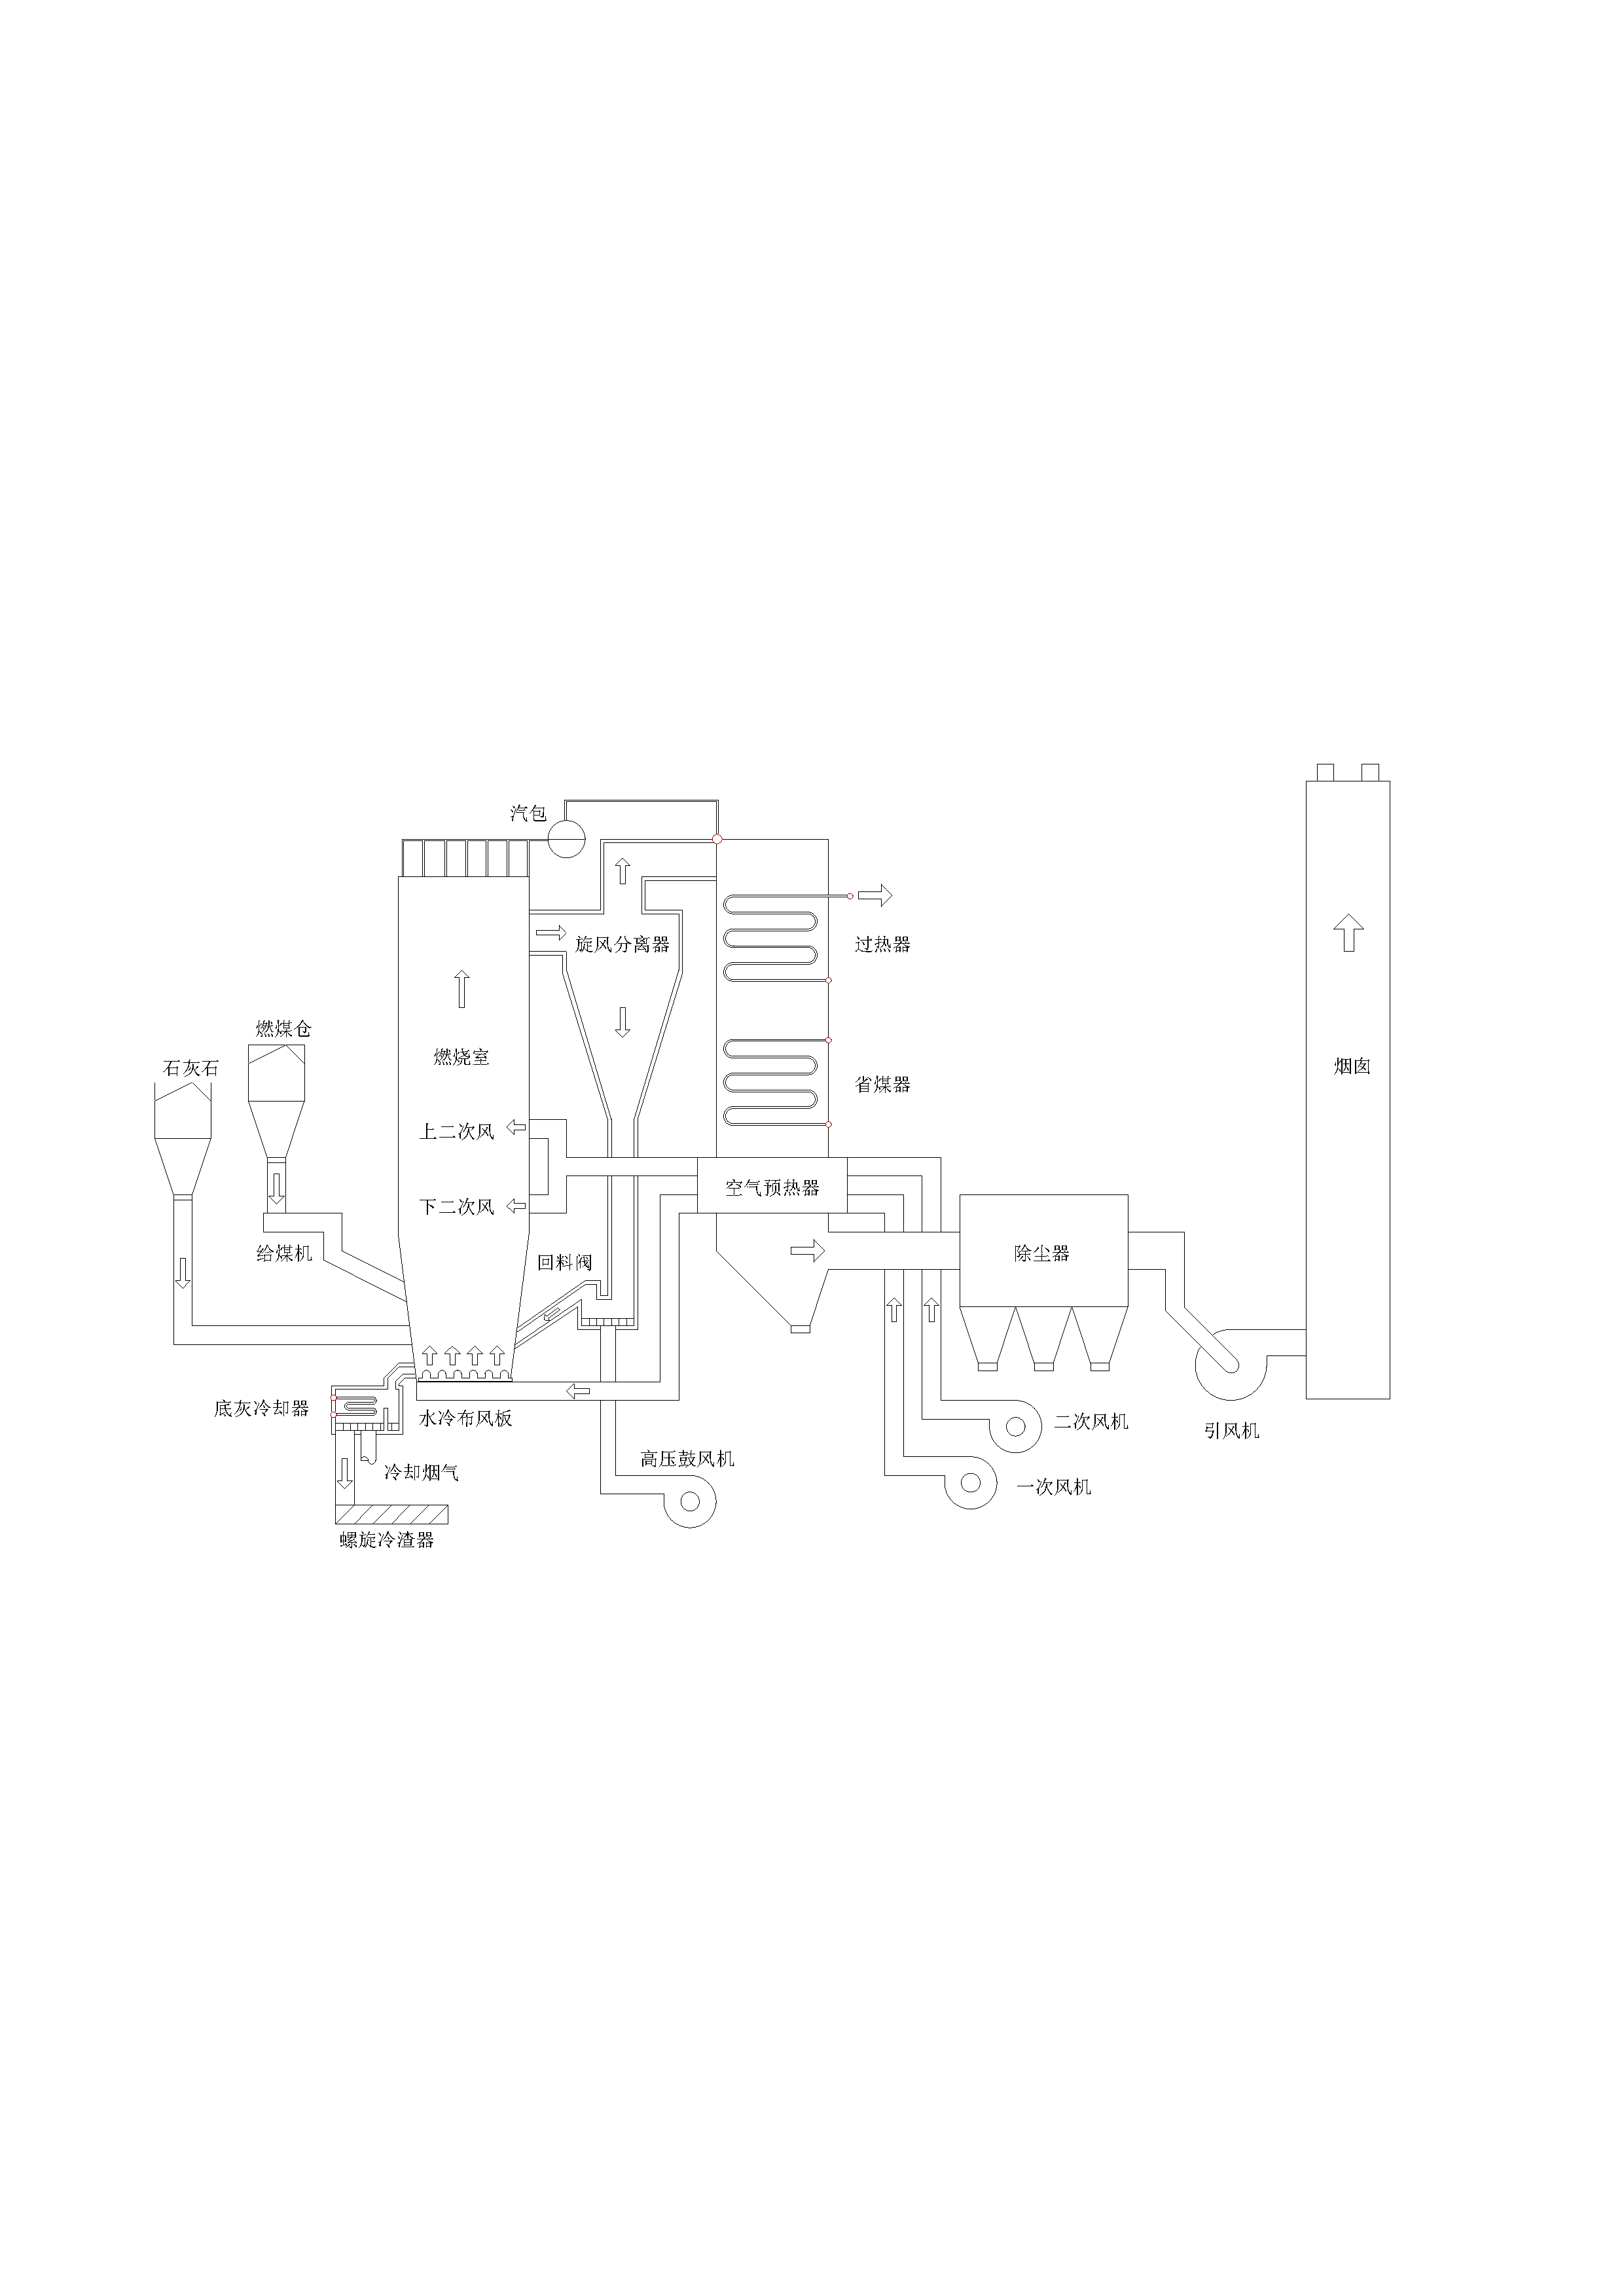
\includegraphics[width=14cm]{cfbb}
\caption{循环流化床锅炉结构示意图} \label{fig:cfbb}
\end{figure}

\subsection{燃烧系统}

循环流化床锅炉的燃烧主要分布在两个区域:炉膛底部的密相区和炉膛上部的稀相区。破碎后的煤粒和脱硫所用的石灰石由给料口送入炉膛,一次风从水冷式布风板进入炉膛。二次风分上下两层分布,由水冷壁前后墙送入炉膛。

锅炉设计有六条输煤线路,每条输煤线路均按25$\,$\si{\percent}~容量设计。如果其中两条皮带损坏,其余四条皮带仍然能够保障给煤,锅炉仍能输出100$\,$\si{\percent}~负荷。石灰石输送线路有三条。通过调整给料机的转速,可以控制锅炉的石灰石量和给煤量。

一次风除了用于维持床料颗粒的流化状态,也提供密相区燃烧所用的氧气。二次风主要作用是进一步补充炉膛内煤粒燃烧所需的氧气。分层分布营造出炉内的密相区和稀相区底部的局部还原性气氛,从而减少~\ce{NOx}生成。在锅炉最大出力工况下,设计一次风占比约为总风量的55$\,$\si{\percent}。

煤粒进入炉膛后,在一次风的作用下流化,在密相区部分燃烧释放热量。与此同时,石灰石在高温下分解生成~\ce{CaO}和~\ce{CO2}。煤中含有的硫燃烧产生的~\ce{SO2}与~\ce{CaO}反应生成~\ce{CaSO4},实现炉内脱硫。未燃尽的煤粒随一次风进入炉膛上部的稀相区,与二次风混合后进一步燃烧,产生大量高温烟气。燃烧产生的烟气携带着床料经炉顶转向,进入旋风分离器进行气-固分离。

被旋风分离器分离出的固态床料则经过J形回料阀返回炉膛实现循环燃烧。燃烧产生的炉渣以及~\ce{CaSO4}经冷渣器排渣口排除锅炉,以维持固定的床层压力。另外,J阀回料器还布置有床料补充口,用于在床料不足时补充床料。


\subsection{汽水系统}

锅炉为自然循环锅炉,水循环采用集中供水,分散引入、引出的方式。给水通过省煤器加热后,集中引入锅筒水空间,并通过集中下降管和下水连接管进入水冷壁下集箱和水冷蒸发屏进口集箱。

水在向上流经炉膛水冷壁、水冷蒸发屏的过程中被加热成为汽水混合物,经各自的上部出口集箱进入锅筒进行汽水分离。被分离出来的水重新进入锅筒水空间,并进行再循环,被分离出来的饱和蒸汽从锅筒顶部的蒸汽连接管引出。饱和蒸汽经低温过热器、屏式过热器和高温过热器后,由高温过热器出口集箱引出。

系统采用喷水减温作为主汽温度调节和保护各级受热面管道的手段。整个过热器系统共布置有两级喷水。一级减温器(左右各一台)布置在低过出口至屏式过热器入口管道上,作为粗调;二级减温器(左右各一台)位于屏式过热器与高温过热器之间的连接管道上,作为微调。


\subsection{风烟系统}

从一次风机鼓出的空气先后经过暖风器、空气预热器加热后分成两路。第一路进入炉膛下部,作为流化风使床料流化,并向上参与炉膛的固体循环;第二路经给煤增压风机增压后,送至六台气力播煤机。从二次风机鼓出的空气也分为两路。第一路先后经暖风器、空气预热器加热后,通过二次风箱进入炉膛参与燃烧;第二路直接作为给煤皮带的密封用风。

烟气及携带的固体粒子离开炉膛通过旋风分离器进口烟道进入旋风分离器。分离后,烟气里的粗颗粒进入J阀,经J阀送回到炉膛。而飞灰仍夹带在烟气中,通过旋风分离器中心筒引出,进入尾部受热面后向下流动。随后高温烟气将热量传递给尾部受热面管内的介质后,通过管式空气预热器进入除尘器。最后,烟气由引风机抽进烟囱,排入大气。

锅炉采用平衡通风,压力平衡点位于炉膛出口。整个风烟系统中均设有调节挡板,运行时便于控制、调节。

\subsection{脱硝系统}

该锅炉采用SNCR(选择性非催化还原法脱硝)技术实现烟气的脱硝处理。浓氨水与稀释水在集箱混合后作为还原剂,喷向旋风分离器出口烟道。在高温环境下,还原剂迅速分解为~\ce{NH3},~\ce{NOx}与~\ce{NH3}反应生成~\ce{N2}和~\ce{H2O}。

在SNCR系统中,影响~\ce{NOx}还原效率的因素有反应温度、氨水与烟气的混合程度、停留时间、烟气中~\ce{NOx}浓度、~\ce{NH3}与~\ce{NOx}~摩尔比、\ce{NH3}逃逸率等等。反应温度应控制在800$\,$\si{\degreeCelsius}~到1000$\,$\si{\degreeCelsius}~之间,反应温度太低会提高~\ce{NH3}逃逸率,反应温度太高则~\ce{NH3}与~\ce{O2}发生反应,不利于脱硝。

\section{现场控制系统简介}
锅炉采用的DCS(Distributed Control System,集散控制系统)为横河电机(中国)有限公司的 CENTUM CS 3000 R3 综合生产控制系统。该系统与用于水/煤灰处理的 GE PLC(Programmable Logic Controller,可编程逻辑控制器)通过 OPC(OLE for Process Control,用于过程控制的对象链接与嵌入)接口接入工厂的 SIS(Supervisory Information System,监控信息系统)。

典型的采用CENTUM CS 3000工厂控制系统的整体结构如图~\ref{fig:cs3000}~所示。CS 3000提供了HIS(Human Interface Station,人机接口站)、现场控制站(Field Control Stations,FCS)、EWS(Engineering workstation,工程师站)、V网和以太网等\cite{konishi2000system}。HIS主要提供操作监视功能,FCS主要负责装置的控制,ENG安装了CS 3000系统生成和维护管理功能,可以进行安装调试。V网是连接FCS、HIS、BCV(总线转化器)等的实时控制总线,具有高速响应性和高可靠性,系统可以通过BCV将其他域的CS 3000、CS 1000、$\mu$~XL系统等接入V网。以太网连接HIS、EWS以及上位信息系统\cite{emori1997communication}。

\begin{figure}[!htb]
\centering
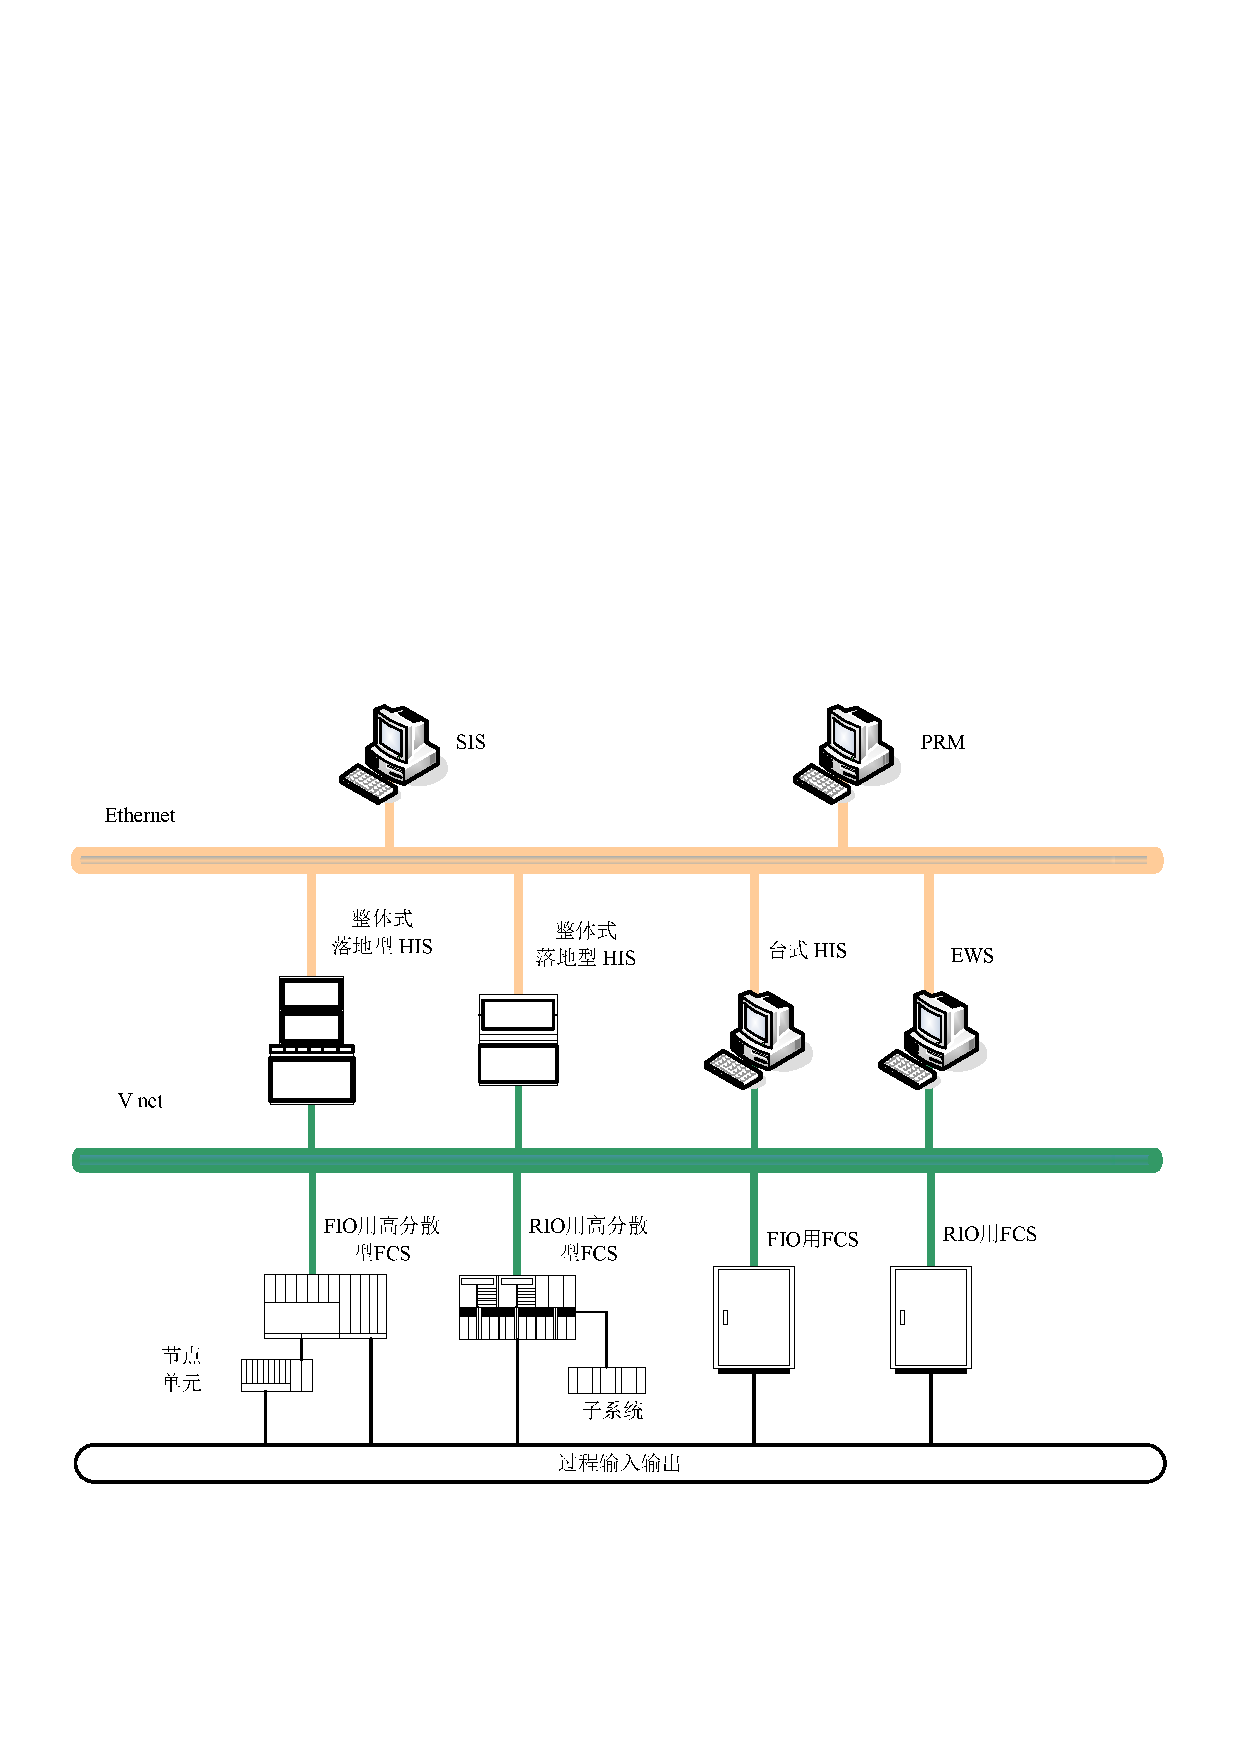
\includegraphics[width=13cm]{cs3000}
\caption{CS 3000架构} \label{fig:cs3000}
\end{figure}

HIS提供了丰富的过程监视/操作功能,除了系统信息和帮助外,还提供了过程报警、过程总貌、趋势图、流程图、顺序表、操作指导等窗口。此外,还提供了报告、画面拷贝等操作支持功能和报表、DDE(Dynamic Data Exchange,动态数据交换)、OPC等扩展功能。

FCS提供了多种执行控制运算的功能块,将连续控制块、顺控块和运算块结合起来即可以流程形式描述控制功能。连续控制块用于过程的监视和控制,主要利用模拟量进行运算处理。顺控块提供顺控功能,使系统按照预先规定的顺序逐步执行控制各阶段的操作。运算块主要作为辅助,提供对模拟信号或者数字信号的通用运算功能。常用的功能块如表~\ref{tab:fcs_blocks}~所示。

\begingroup
\renewcommand*{\arraystretch}{1.67}
\begin{small}
\begin{longtable}[!h]{l|p{11cm}}
% 首页表头
\caption[FCS常用控制块]{FCS常用控制块} \label{tab:fcs_blocks}\\

\toprule[0.5pt]
\hline
名称  & 说明 \\
\midrule
\endfirsthead
% 续页表头
\caption[FCS常用控制块(续)]{FCS常用功能块(续)} \\
\toprule[0.5pt]
\hline
名称  & 说明 \\
\midrule
\endhead
% 首页表尾
\hline
\multicolumn{2}{r}{\small 续下页}
\endfoot
% 续页表尾
\hline
\bottomrule[0.5pt]
\endlastfoot

PVI &   将输入信号作为测量值(PV)进行显示\\
PVI-DV  &   除PVI的功能外,还有“偏差报警查”以及“设定值限制器”2种功能。\\
PID &   对于测量值和设定值的偏差进行比例(P)、积分(I)、微分(D)的控制动作\\
MLD&输出设定的操作输出值(MV),在手动操作调节阀等使用\\
MLD-PVI&MLD-PVI块进行测量值(PV)和操作输出值(MV)的输出。一边监视测量值(PV),一边对操作端进行手动操作\\
MLD-SW&切换选择来自调节块等的输出信号和自身的手动操作输出信号\\
VELLIM&将变化量限制在变化率限制值内后输出,避免信号发生突变\\
FOUT&将从具有调节功能的功能块输入的串级信号分配给位于串级控制回路的下游的多个调节块中\\
LC64&用逻辑运算元件记录输入信号和输出信号的关系\\
RL&判定2个数据间的大小关系或者逻辑积\\
AVE&求输入数据的平均值\\
ADD&执行加法运算处理及减法运算处理\\
MUL&执行乘法运算\\
AND&在运算运算输入值(RV1,RV2)的逻辑积\\
NOT&执行否定运算处理\\
OR&运算运算输入值(RV1,RV2)的逻辑和\\
TON&在运算输入值(RV)由0变化为其它值时,只在1次扫描之间把运算输出值(CPV)设定为1\\
OND&在运算输入值(RV)由0变化为其它值后,设定时间(STM)经过后,将运算输出值(CPV)设为1\\
LAG&对输入信号执行1步滞后处理\\
CALCU&定义任意运算算法\\
DSET&输出由操作监视功能输入的任意工业单位数据\\
\end{longtable}
\end{small}
\endgroup
CS 3000提供的工程技术功能既可以与HIS共存,也可以独立安装在通用PC上, 其基本功能由系统视图和组态构成。组态提供了对项目通用功能、操作监视、控制功能进行生成的能力。用户还可以利用调试功能对工程进行运行前的确认。


\section{燃烧系统控制现状}

现场DCS虽然有PID和手动控制两种控制手段,但实际上由于PID参数很久没有重新整定,燃烧系统大部分时段处于手动控制状态。

\subsection{主汽压力回路}

除了锅炉启动和停炉外,当锅炉正常运行时,维持合格的主蒸汽压力是燃烧系统的首要目标。对于该锅炉而言,最大出力状态下,正常的过热器出口蒸汽压力应维持在9.81$\,$\si{\mega\pascal}~$\pm$~0.1$\,$\si{\mega\pascal}。当锅炉负荷改变时,可以通过调节给煤量和风量来调节锅炉负荷。
 
目前主汽压力的控制与煤粉炉类似,都是通过调节给煤量来实现的,采用主汽压力—给煤量串级调节和PID控制器,如图~\ref{fig:gas_pre_pid}。在该串级控制回路中,主回路控制主汽压力,副回路控制给煤量,副回路并不比主回路响应迅速。此外,锅炉的主汽流量会对主汽压力产生较大影响,该控制策略并没有考虑主汽流量的影响。
\begin{figure}[!htb]
\centering
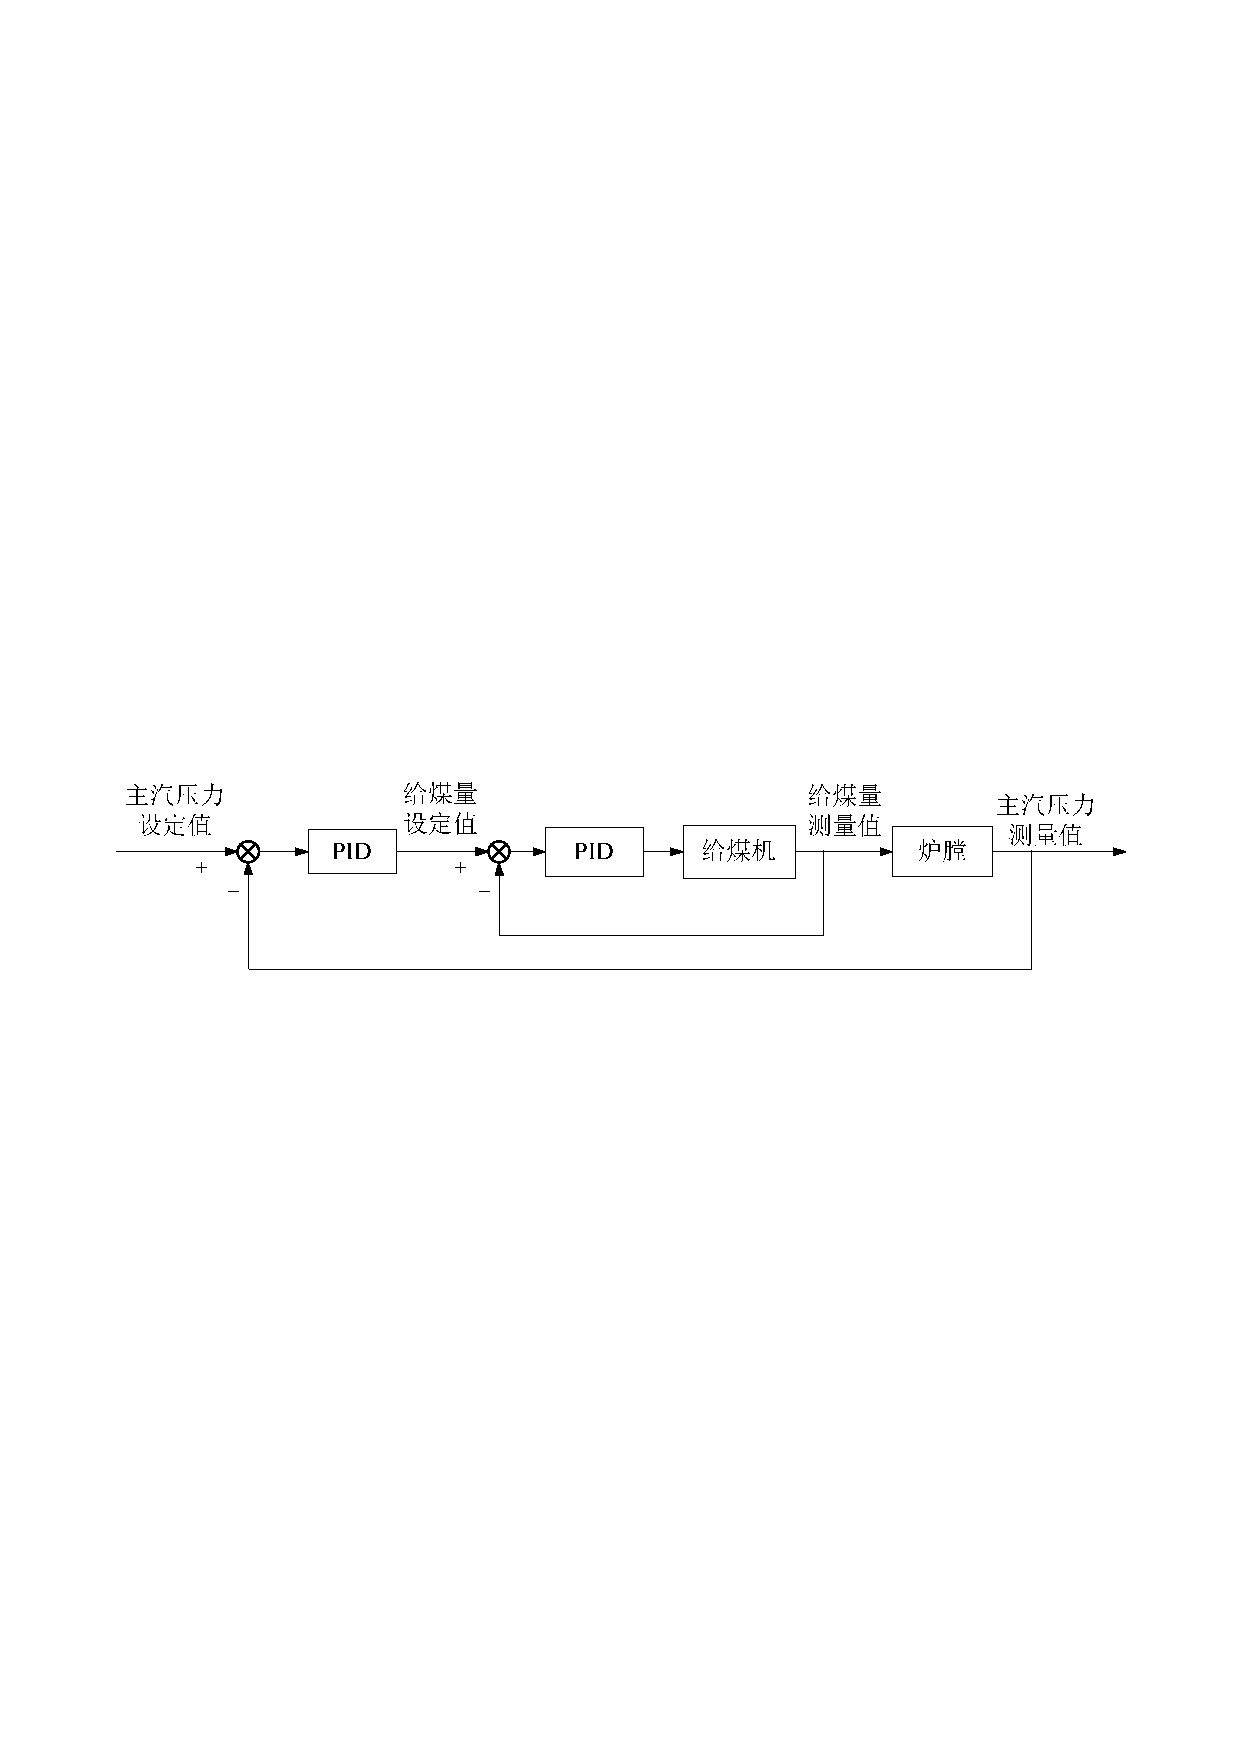
\includegraphics[width=13cm]{gas_pre_pid}
\caption{主汽压力回路PID控制策略} \label{fig:gas_pre_pid}
\end{figure}

图~\ref{fig:gas_pre_line_pid}~为某天主汽压力的变化曲线,可以看出主汽压力的波动非常大,在部分时刻甚至达到了0.3$\,$\si{\mega\pascal}。国标要求主汽压力的波动应在设定值上下0.1$\,$\si{\mega\pascal}~内,这样的运行状态会导致下游发电机运行不稳定,甚至导致生成事故。

\begin{figure}[!htb]
\centering
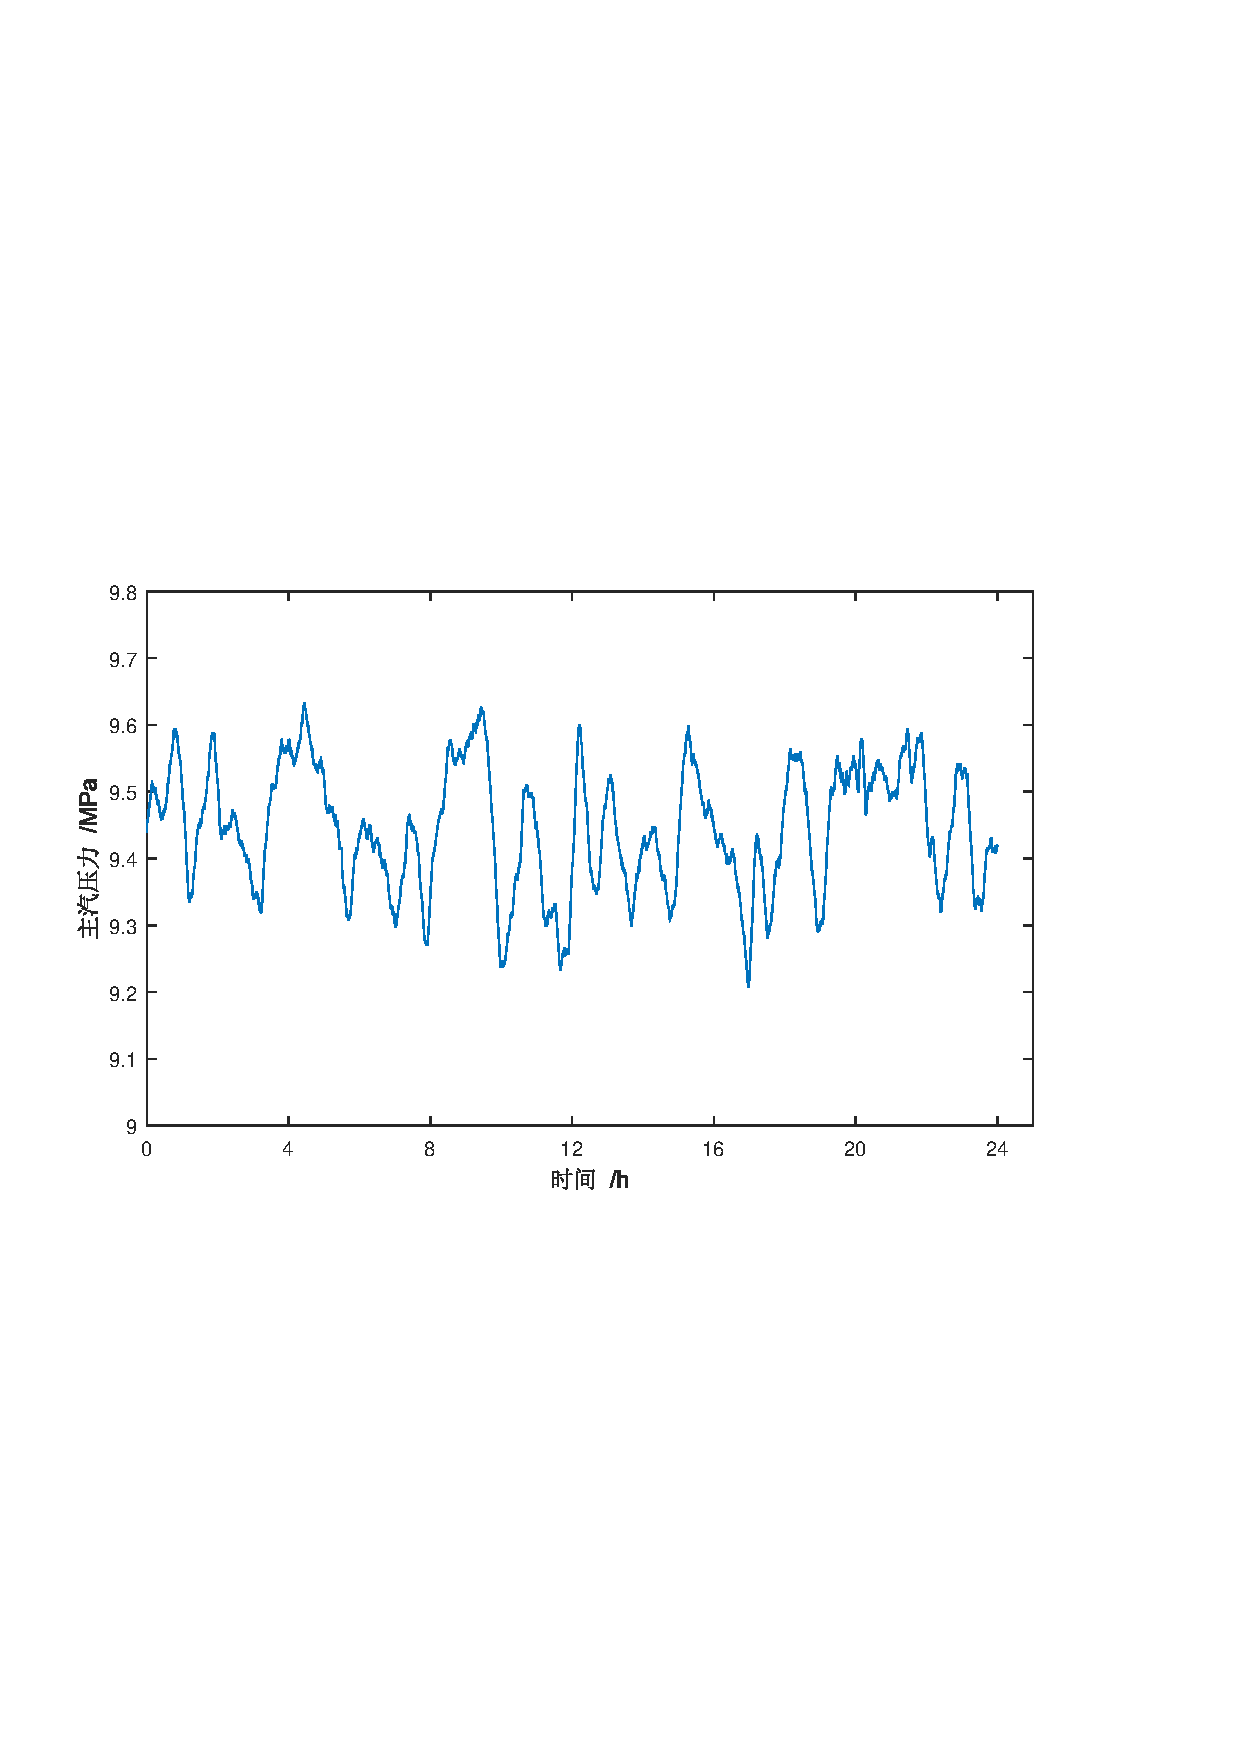
\includegraphics[width=12cm]{gas_pre_line_pid}
\caption{主汽压力回路控制效果} \label{fig:gas_pre_line_pid}
\end{figure}
 
\subsection{床温回路}
床温由24只床温热电偶测量,平均后作为床温信号。正常的床温范围在850$\,$\si{\degreeCelsius}~到935$\,$\si{\degreeCelsius}~之间,并且允许短时间内的大幅变化,以此来满足快速调节锅炉负荷的要求。但当达到所需负荷后,床温应当重新稳定在设定值附近。床温的设定值对循环流化床锅炉的运行有较大影响。床温过高,虽然会提高锅炉的热效率,但高床温会导致燃烧生成更多的~\ce{NOx},影响石灰石脱硫剂的脱硫效率,甚至导致炉膛内床料结焦,床层不能维持良好的流化状态,影响燃烧的持续稳定进行。床温过低会导致燃烧不完全,甚至锅炉灭火。
 
目前床温的控制是通过一次风来实现的,采用床温—一次风量的串级回路和PID控制器,如图~\ref{fig:bed_tem_pid}。单独使用一次风控制床温存在这样的问题:调节幅度小的话控制效果不明显;调节幅度大了则可能因为一次风和给煤量不匹配而影响到流化状态,也存在给煤没有快速跟导致上炉温上升后又快速回落的问题。
\begin{figure}[!htb]
\centering
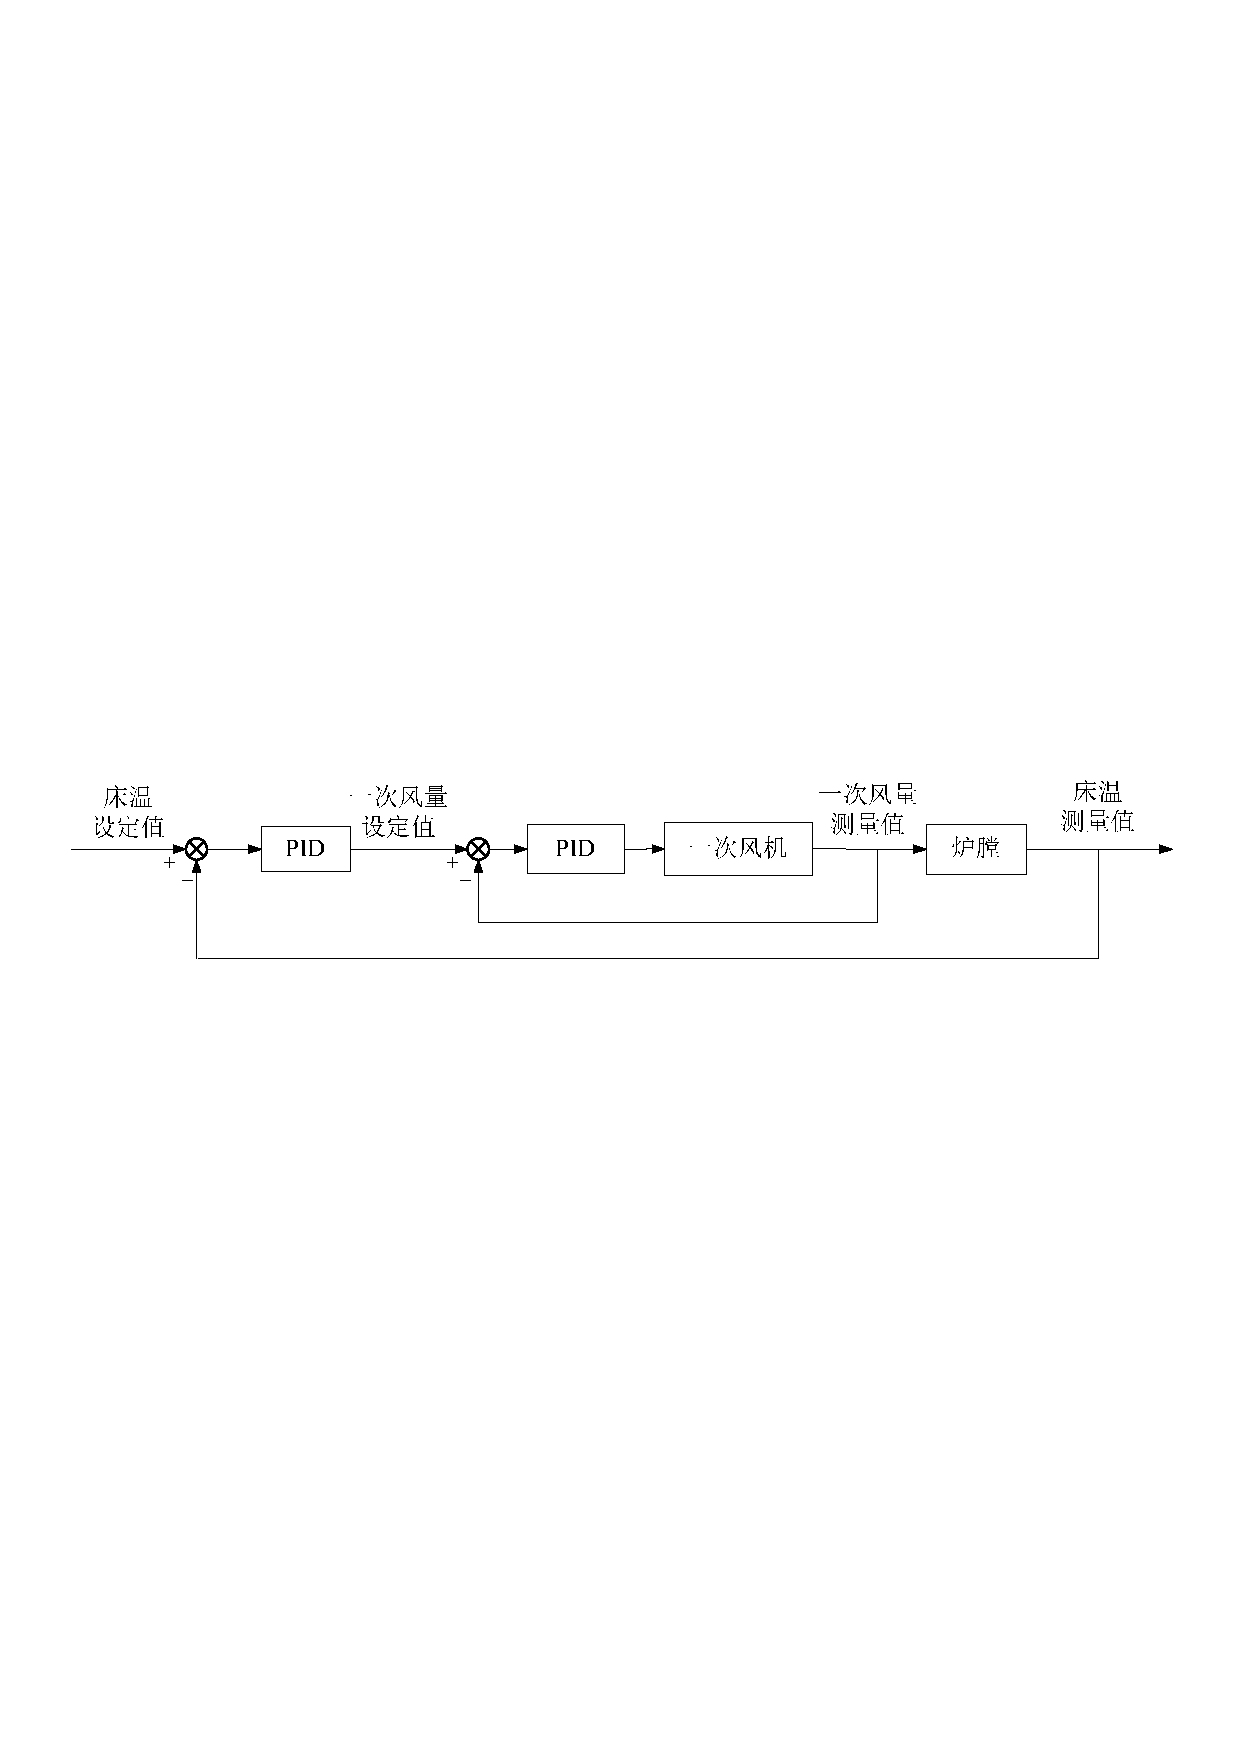
\includegraphics[width=13cm]{bed_tem_pid}
\caption{床温回路PID控制策略} \label{fig:bed_tem_pid}
\end{figure}

\begin{figure}[!htb]
\centering
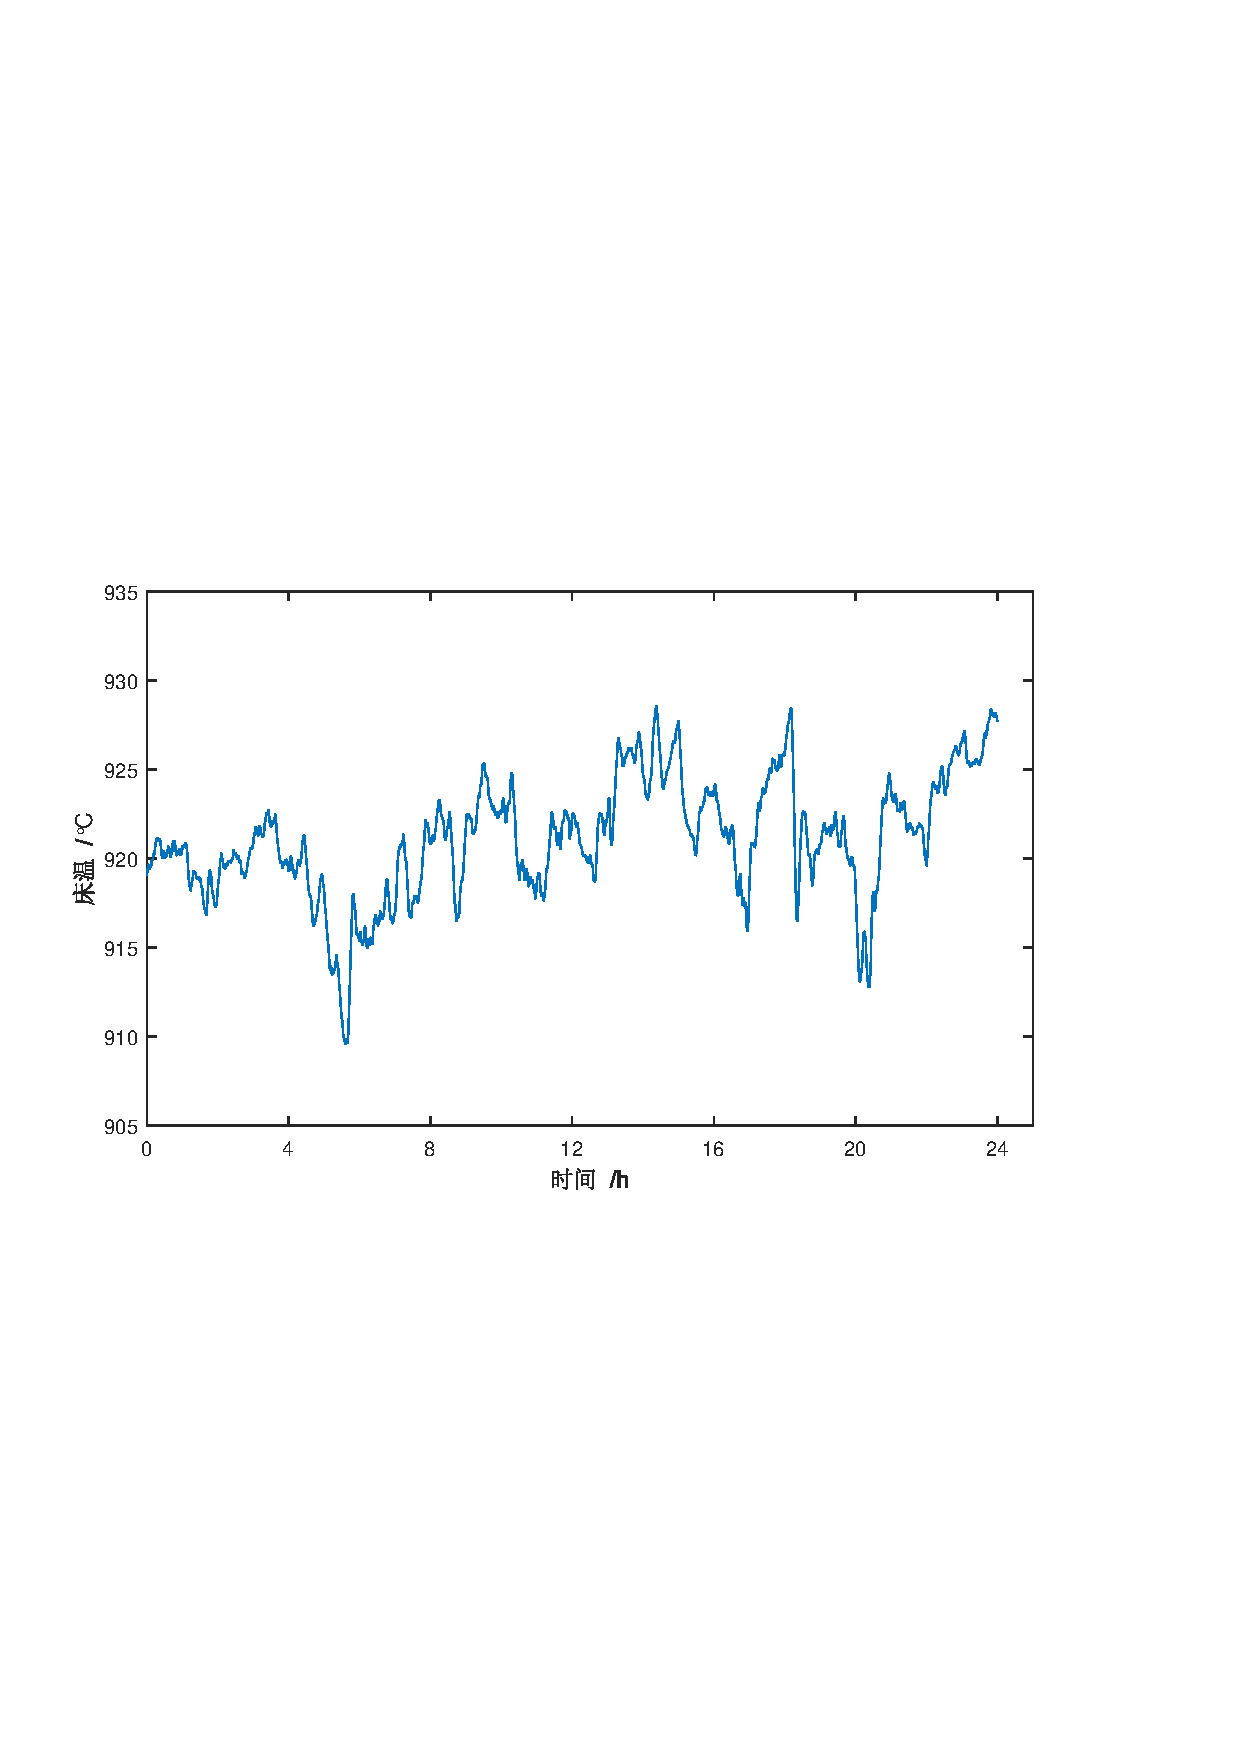
\includegraphics[width=12cm]{bed_tem_line_pid}
\caption{床温回路控制效果} \label{fig:bed_tem_line_pid}
\end{figure}
 
某日床温曲线如图~\ref{fig:bed_tem_line_pid}~所示。床温基本维持在910$\,$\si{\degreeCelsius}~到930$\,$\si{\degreeCelsius}~之间。但是床温一直处于较大波动状态。在约4时床温开始下降,直到910$\,$\si{\degreeCelsius},,随后又开始快速上升到920$\,$\si{\degreeCelsius},之后床温开始出现较大程度的振荡。在18时床温达到了930$\,$\si{\degreeCelsius},接近高限935$\,$\si{\degreeCelsius},随后又在20时下降到910$\,$\si{\degreeCelsius}。



\subsection{床层压差回路}

床层压差反映了循环流化床密相区的床料厚度。循环流化床锅炉的正常运行要求维持一定的床层厚度。料层过薄,料层容易被流化风吹穿产生沟流,进而导致流化不均匀引起局部结渣。同时也会导致灰渣含碳量高,燃烧不完全,降低锅炉的热效率。料层过厚会引起水冷风室压力过高,密相区底部大颗粒物料堆积,堵塞流化风压头,危及锅炉的安全运行。由于炉膛内处于流化状态,没有明显的料位高度,床层厚度只能通过床层压差及一次风量估算。锅炉正常运行情况下,床层厚度应保持500$\,$\si{\mm}~左右,床层压差应保持在5$\,$\si{\kilo\pascal}~到10$\,$\si{\kilo\pascal}。
 
目前床层压差的控制是通过调节冷渣机转速来实现的,采用单回路调节,控制器为PID控制器,如图~\ref{fig:bed_pre_pid}。没有考虑给煤量和石灰石量对床层压差的影响。在给煤量波动不大时,这个回路是没有什么问题的。但当给煤量和石灰石量波动较大时,单纯依靠冷渣机转速来控制床层压差,床层压差会出现较大波动。

\begin{figure}[!htb]
\centering
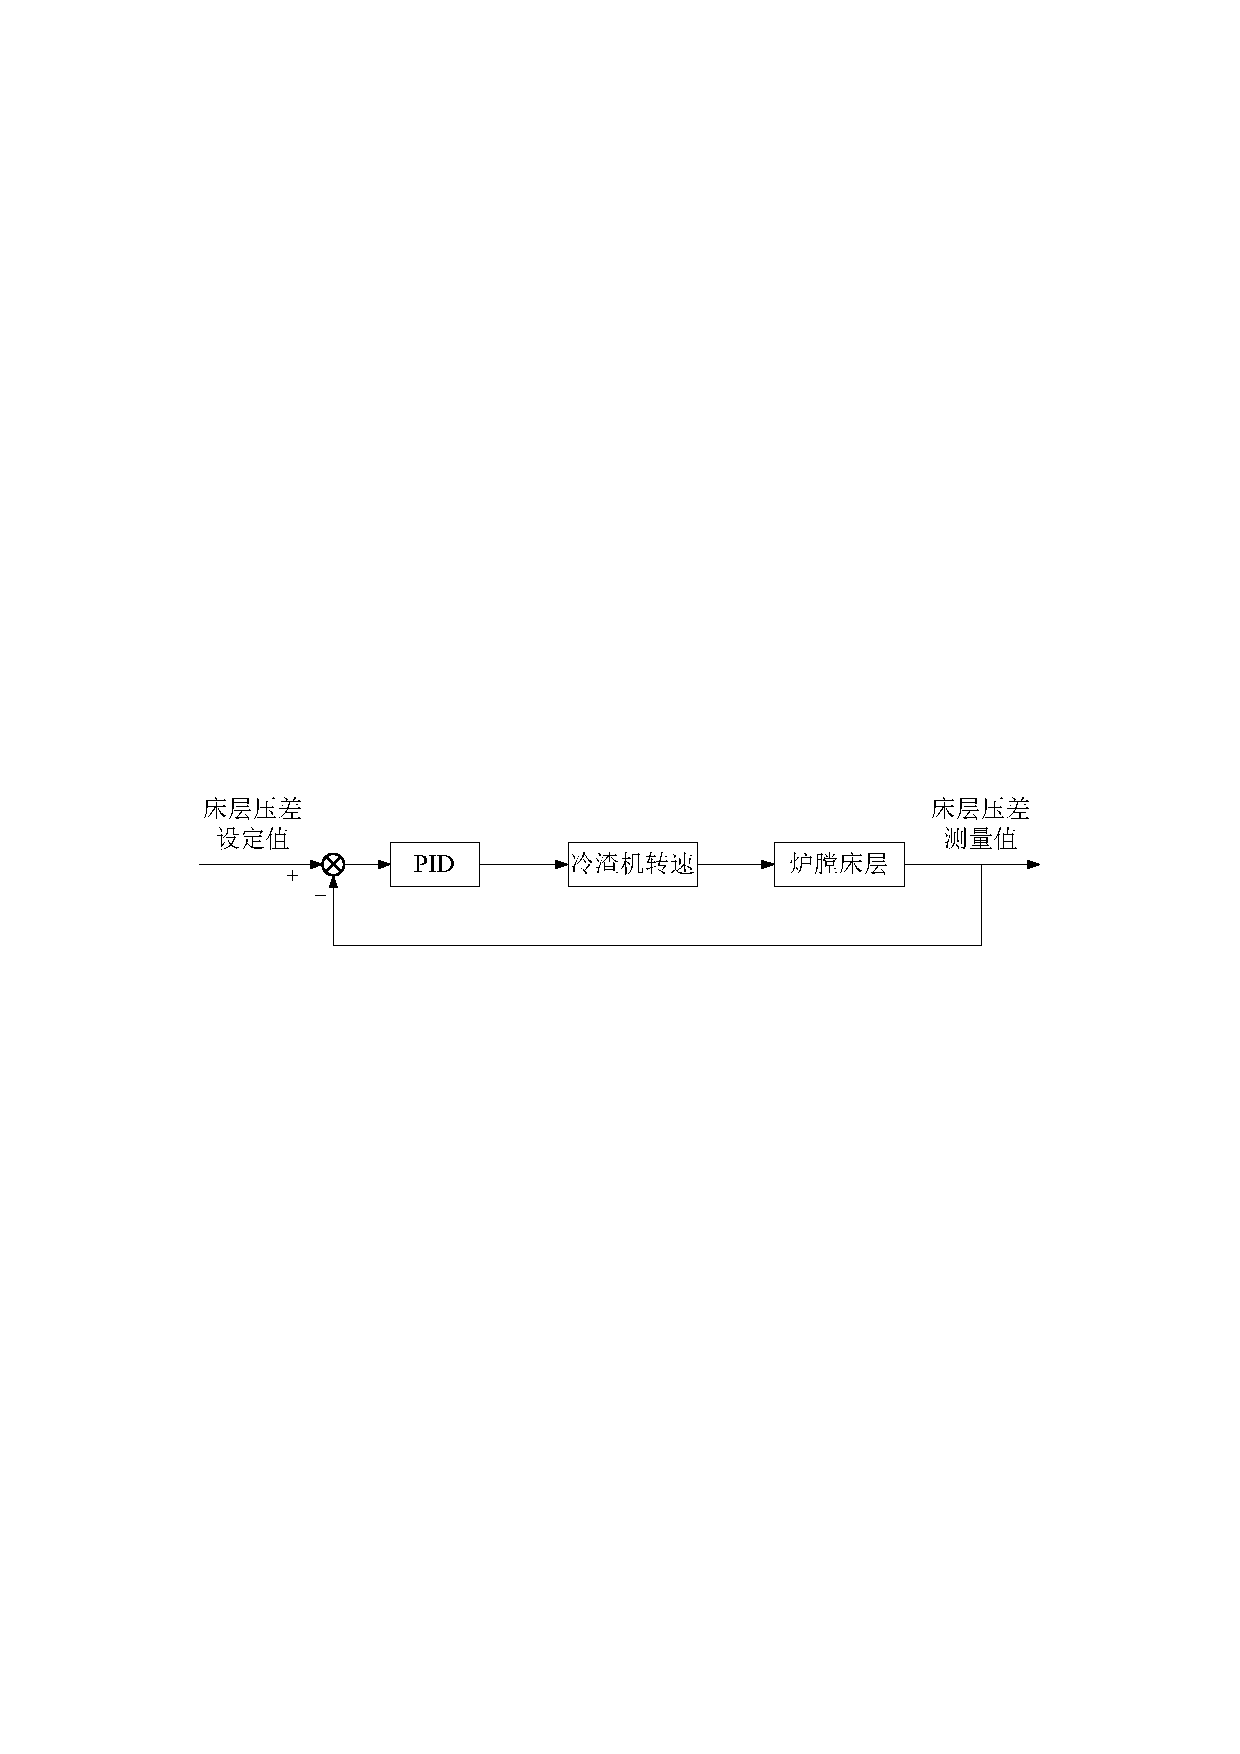
\includegraphics[width=13cm]{bed_pre_pid}
\caption{床层压差回路PID控制策略} \label{fig:bed_pre_pid}
\end{figure}


\begin{figure}[hbtp]
\centering
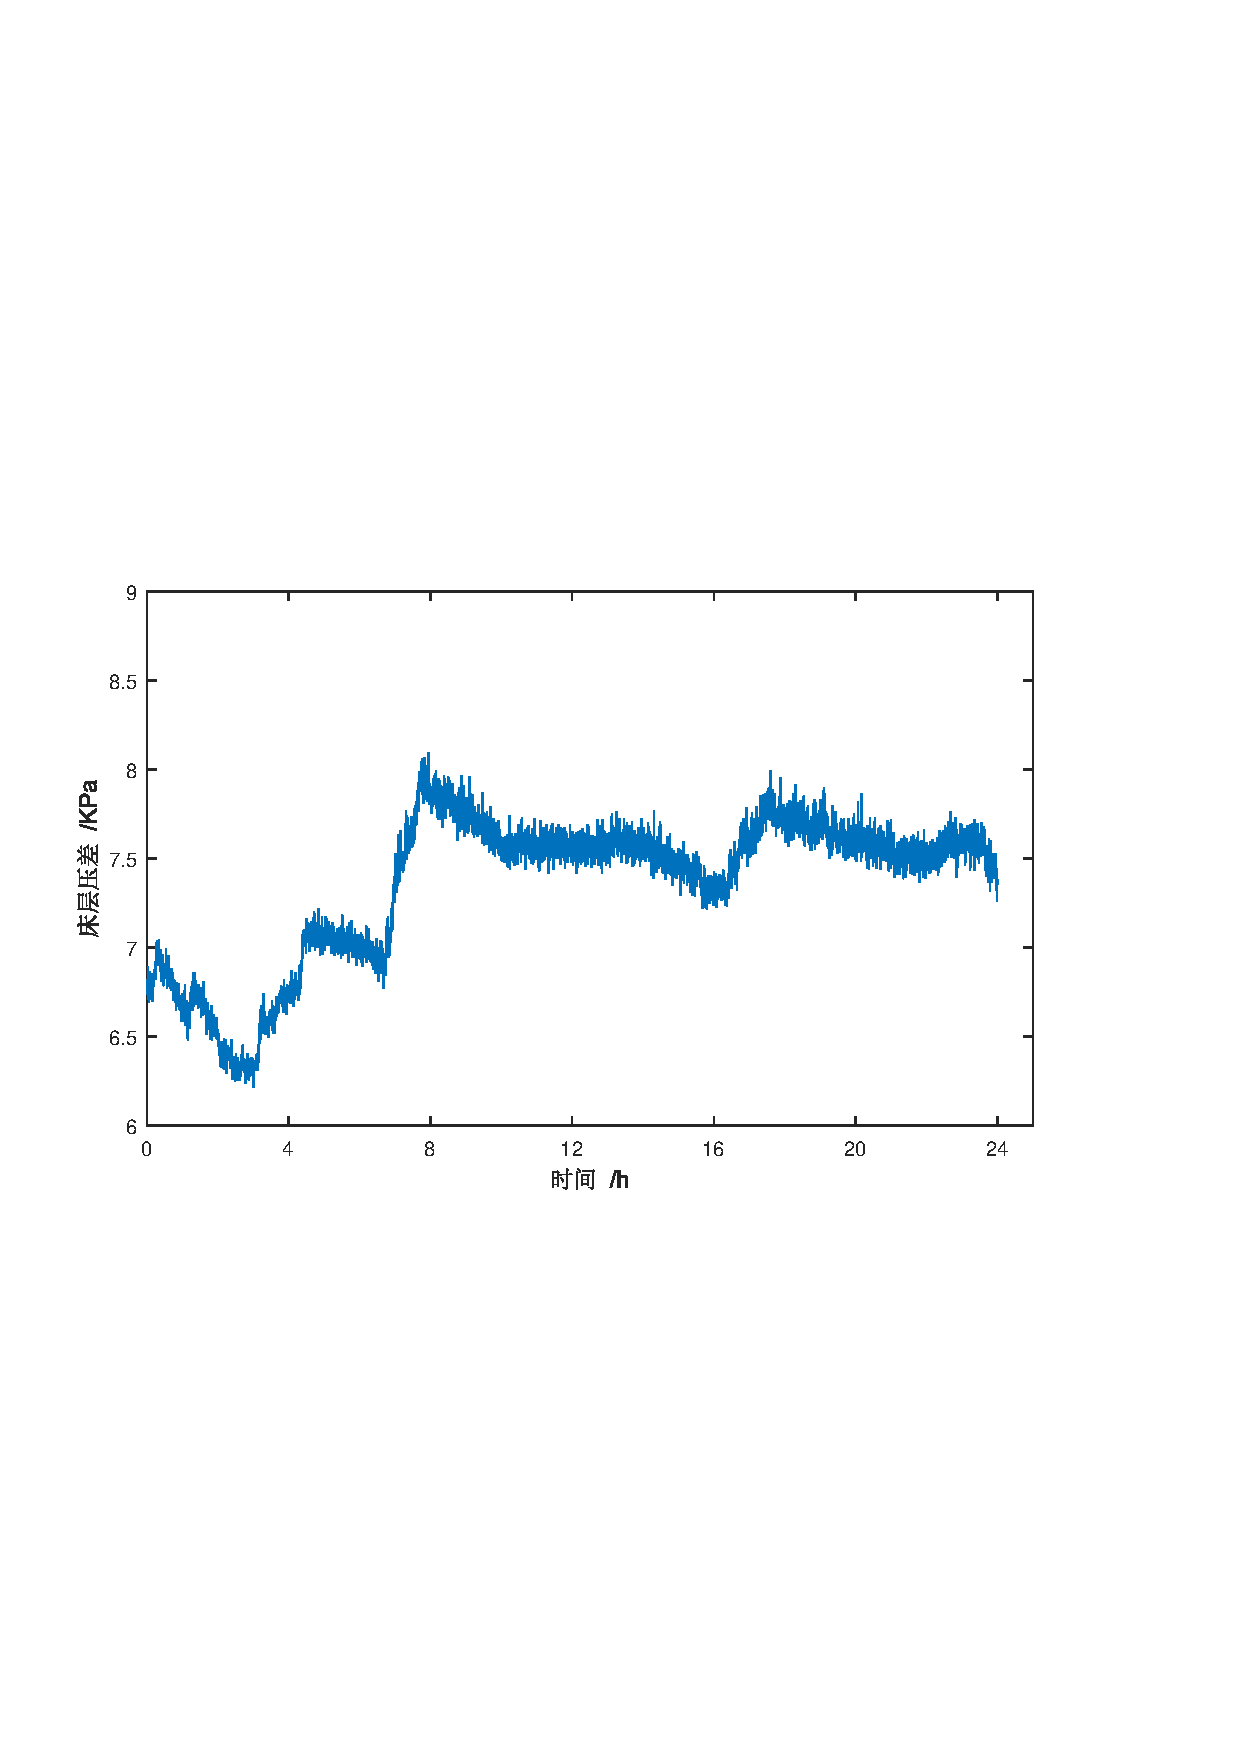
\includegraphics[width=12cm]{bed_pre_line_pid}
\caption{床层压差回路控制效果} \label{fig:bed_pre_line_pid}
\end{figure}
 
某日床层压差曲线如图~\ref{fig:bed_pre_line_pid}~所示。可以看出全天床层压差的波动幅度2$\,$\si{\kilo\pascal}~左右。从开始床压下降到6.2$\,$\si{\kilo\pascal}~,调节到7.2$\,$\si{\kilo\pascal}~后又出现压差的下滑的趋势,随后调节到8.2$\,$\si{\kilo\pascal}~后压差再次下滑,基本上不断向上调节,又不断下滑。虽然生产工艺允许压差的较大幅度波动,但失控的压差容易导致床层流化状态的不稳定,增加燃烧系统的控制难度。


\section{氮氧化物测量现状}
\label{sec:nox_measure_now}
\ce{NOX}是燃煤电站排放的主要污染物之一。在脱硝系统中,系统通过调节氨水和稀释水的流量来控制~\ce{NOx}浓度,氨水和稀释水的流量是由烟道~\ce{NOx}测定值与~\ce{NOx}设定值的偏差计算的。因此,烟道~\ce{NOx}排放量的测量对脱硝控制有着重要影响。除此之外,~\ce{NOx}测量的准确性也会影响燃煤电厂脱硝电价的核算。


~\ce{NOx}由~\ce{NO}和~\ce{NO2}组成,因此其测量也依托于~\ce{NO}和~\ce{NO2}的测量技术。~\ce{NO}的测量主要依靠化学发光法,~\ce{NO2}的测量主要依靠湿化学法和光谱法。这些方法测定灵敏度高、检出限低,但测量过程需要将~\ce{NOx}完全转化为~\ce{NO}或~\ce{NO2},装置复杂,价格昂贵,且测量耗时较长。相对而言,~\ce{NOx}化学传感器能满足工业现场连续监测的要求。根据测量原理,~\ce{NOx}化学传感器又分为声表面波~\ce{NOx}化学传感器、~\ce{NOx}光纤化学传感器、半导体~\ce{NOx}化学传感器和~\ce{NOx}电化学传感器\cite{王康丽2003氮氧化物化学传感器}。

\begin{figure}[hbtp]
\centering
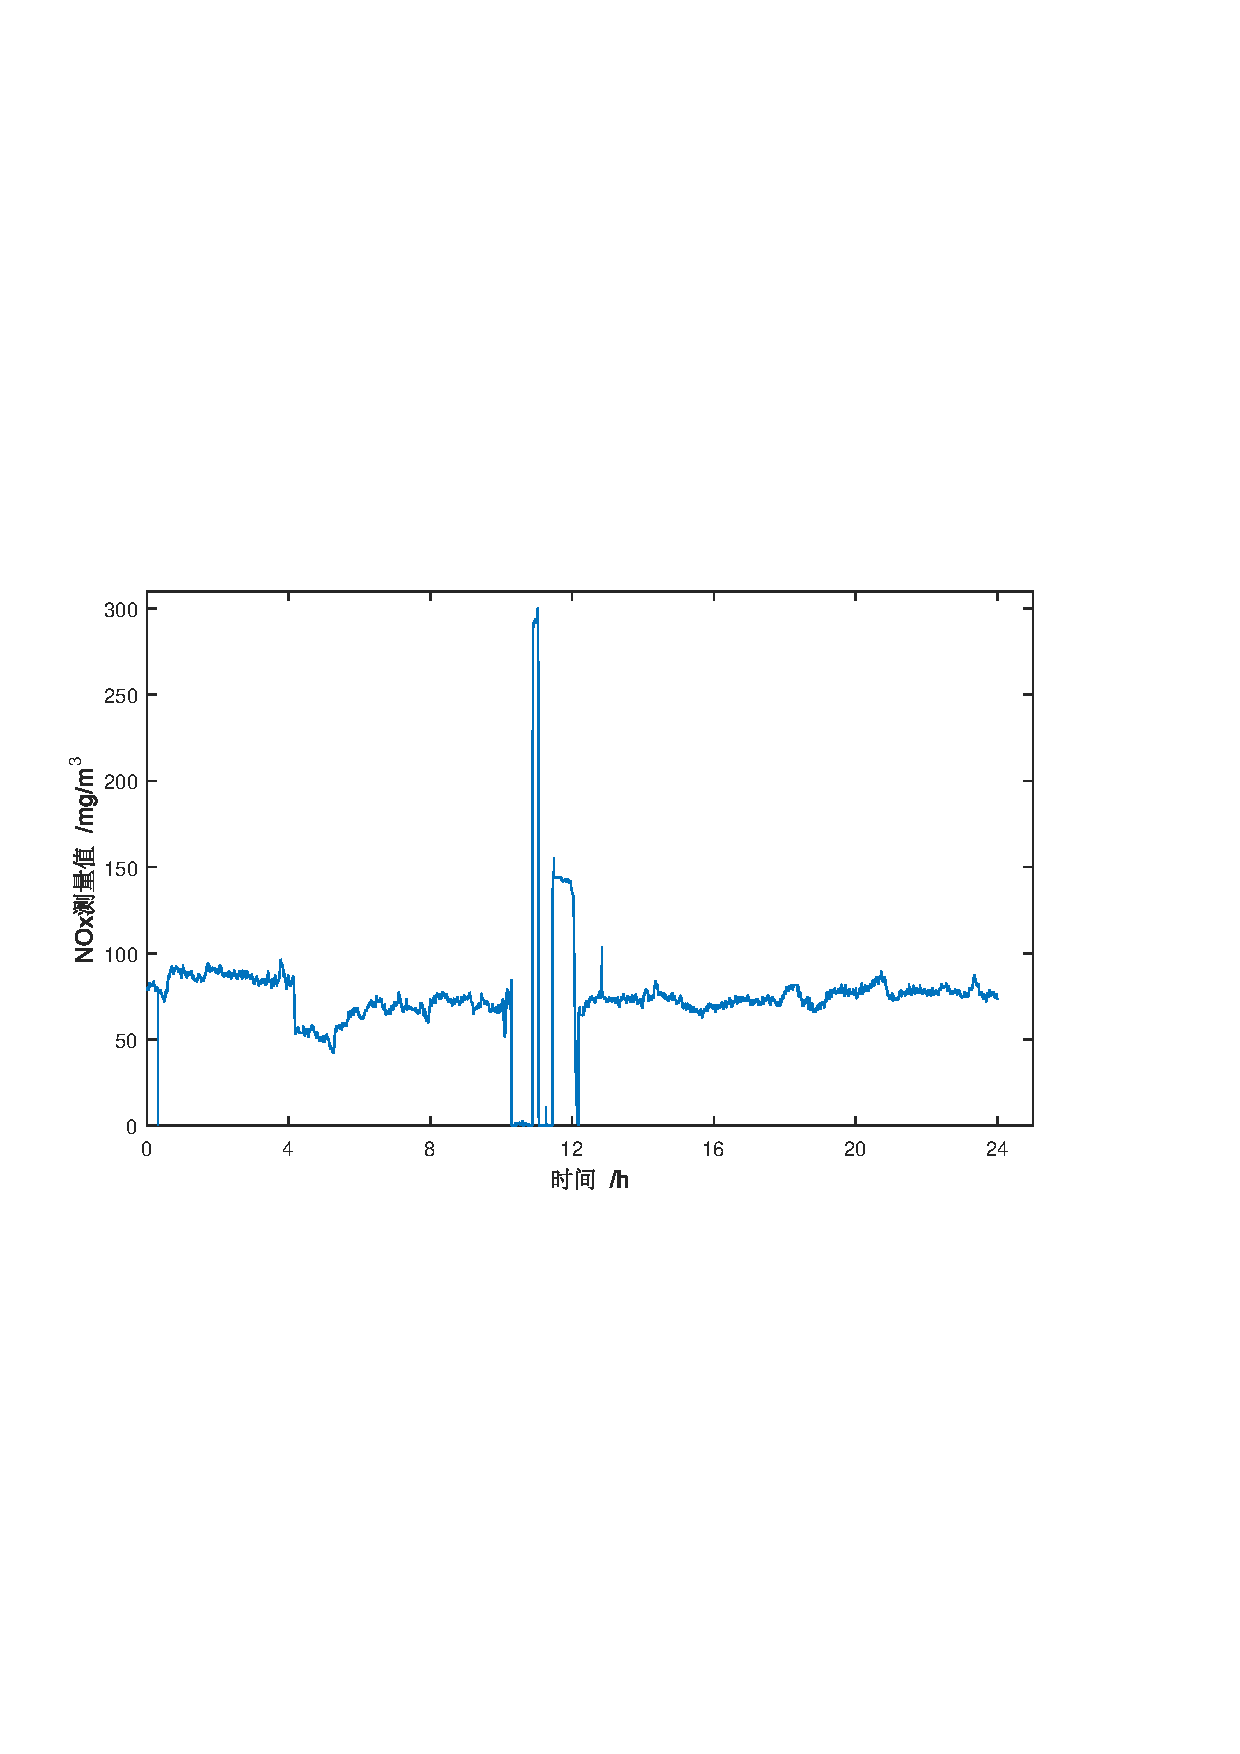
\includegraphics[width=12cm]{nox_measure}
\caption{现场~\ce{NOx}测量现状} \label{fig:nox_measure}
\end{figure}

独山子热电厂采用氧化锆探头作为~\ce{NOx}测量装置,该传感器属于固态电解质电化学传感器,选择专一性好且结构紧凑,适用于工业现场连续监测。但由于氧化锆材料的稳定性和工业现场复杂工作环境,存在性能劣化、机械性差、电势异常、电极脱落、寿命短等问题\cite{罗顺安2010氧化锆}。分析DCS系统记录的历史数据可以发现,~\ce{NOx}传感器的故障往往导致脱硝回路的异常运行。如图~\ref{fig:nox_measure}~所示,~\ce{NOx}传感器出现了三次故障,故障时段~\ce{NOx}测量值记录为0,故障时间长达1$\,$\si{\hour}。由于传感器发生故障,脱硝装置运行异常,导致当日部分时段~\ce{NOx}排放量达到了300$\,$\si[per-mode=symbol]{\mg\per\m^3},是国家规定限定值的3倍。


 
因此,有必要改进现场~\ce{NOx}测量方法,尽可能避免传感器故障对脱硝系统的影响。

\section{本章小结}
本章首先简要介绍了现场循环流化床锅炉的设计参数、结构、运行工艺和DCS系统。随后分析了当前燃烧系统的控制策略和控制水平,可以看出控制策略存在一定的问题,原有的自动控制系统基本失效,燃烧系统处于手动控制状态。最后结合现场实际测量数据分析了~\ce{NOx}传感器存在的问题,指出提高其测量水平的必要性。